\chapter{La compilation}
\section{Compilation des $\lambda$-termes en termes applicatifs}
Il existe un formalisme appelé \textit{Logique Combinatoire} qui permet de construire
un calcul sans variables liées. 
C'est surprenant, mais ces variables liées qui sont introduites par abstraction puis éliminées par application
ne sont finalement pas essentielles pour le calcul.

Comment traduire une abstraction en termes applicatifs ? 
Nous allons définir une traduction $M\mapsto  M_@$ , ainsi qu'une traduction en sens inverse
$A\mapsto A_\lambda$.

L'idée est de partir sur les règles de traduction suivantes :
\[
\begin{array}{lcl}
	\lceil \lambda x . x \rceil &=& I \\
	\lceil \lambda x . M \rceil &=& K M \quad (x \notin M) \\
	\lceil \lambda x . M N \rceil &=& S \lceil \lambda x . M \rceil \lceil \lambda x . N \rceil \quad (x \in M,N) \\
\end{array}
\]
où $ \lceil T \rceil$ représente le $\lambda$-terme $T$ sans lambda abstraction. 

Nous serions tentés de vouloir faire directement la traduction en utilisant ces règles.
Il nous faut cependant passer par un opérateur d'abstraction $A \mapsto [x].A$ qui permettra de "supprimer" toutes 
les lambdas en profondeur dans le $\lambda$-terme, puis seulement ensuite, nous pourrons utiliser les trois règles ci-dessous:
\[
\begin{array}{lcl}
	{[x]}  . x   &\equiv & I \\
	{[x]} .  A   &\equiv & K A \quad (x \notin A) \\
	{[x]}  . A B &\equiv & S ([x] . A)([x] . B)  \quad (x \in A,B) \\
\end{array}
\]

Les combinateurs $I, K$ et $S$ sont définis comme ceci:
\[
\begin{array}{ccc}
	I &=& \lambda x . x \\
	K &=& \lambda x y . x \\
	S &=& \lambda x y z . x z (y z) \\
\end{array}	
\]

Et voici la définition de la traduction des $\lambda$-termes en termes applicatifs.
\[
\begin{array}{lcl}
	 (x)_@  &\equiv & x \\
	(PQ)_@  &\equiv & (P)_@ (Q)_@ \\
	(\lambda x.M)_@  &\equiv & [x] .(M)_@   \\
\end{array}
\]

Dans la définition de notre type applicatif \verb+ski+, nous incluons aussi notre opérateur $[x].A$ 
avec le constructeur \verb+Op+.

\begin{Verbatim}
type ski = 
| Varia of string
| I
| K
| S
| Appl of ski*ski 
| Op of string * ski ;;

exception SkiExec

let rec lambda_ski = function
| Lam(x, t) -> lambda_ski_op (Op(x, lambda_ski t))
| Var(x) -> Varia(x)
| App(m,n) -> Appl(lambda_ski m, lambda_ski n) 
and lambda_ski_op = function
| Op(x,Varia y) when x=y -> I 
| Op(x, t) when not (mem x (var t)) -> Appl(K, t) 
| Op(x, Appl(m, n))  when (mem x (var m)) || (mem x (var n)) 
	  -> Appl(Appl(S, (lambda_ski_op (Op(x,m)))), (lambda_ski_op (Op(x,n)))) 
| _ -> raise SkiErreur
\end{Verbatim}
A titre d'exemple, traduisons notre combinateur $y$ en termes applicatifs:
\begin{Verbatim}
utop # print_ski (lambda_ski y) ;;
((S((S((S(KS))((S(KK))I)))(K((SI)I))))((S((S(KS))((S(KK))I)))(K((SI)I))))
\end{Verbatim}
Une fois le code compilé, son exécution sera réalisée avec les règles de réécriture :
\[
\begin{array}{ccc}
	Ix &\longrightarrow & x \\
	Kxy &\longrightarrow & x \\
	Sxyz &\longrightarrow & x z (y z)	\\
\end{array}	
\]
Voici une première version de l'exécution de ces règles de réécriture. Ce code un est peu bourrin car on appelle
la fonction tant que le terme n'est pas réduit.
\begin{Verbatim}
let rec exec_aux = function
| Appl(I, x) -> exec_aux x
| Appl(Appl(K, x), y) -> exec_aux x
| Appl(Appl(Appl(S,x),y),z) -> Appl(Appl(exec_aux x, exec_aux z), Appl(exec_aux y,exec_aux z))
| Appl(x,y) -> Appl(exec_aux x, exec_aux y)
| Varia x -> Varia x
| I -> I
| K -> K
| S -> S
| _ -> raise SkiErreur 
and  exec t =
let r = exec_aux t in
	if r=t then r else exec_aux r 
\end{Verbatim}

Voici une version plus élégante qui retourne la forme réduite.
\begin{Verbatim}
let rec ski_norm m =
match m with
| S | K | I -> m
| Varia x -> m
| Appl (m0, m1) ->
match ski_norm m0 with
| I -> ski_norm m1
| Appl (K, m') -> m'
| Appl (Appl (S, m3), m2) -> ski_norm (Appl (Appl (m3, m1), Appl (m2, m1)))
| autre -> Appl (autre, ski_norm m1);;
\end{Verbatim}

La traduction en sens inverse $A \mapsto A_\lambda $ se fait naturellement par la fonction ML ci-dessous:
\begin{Verbatim}
let rec ski_lambda = function
| I -> Lam("x", Var "x")
| K -> Lam("x", Lam("y", Var "x"))
| S -> Lam("x", Lam("y", Lam("z", App(App(Var "x", Var "z"), App(Var "y", Var "z")))))
| Varia(x) -> Var(x)
| Appl(m,n) -> App(ski_lambda m,ski_lambda n)
| _ -> raise SkiErreur
\end{Verbatim}

Utilisons l'exemple de la factorielle, exemple complexe car il comporte les représentations en $\lambda$-termes
du combinateur $Y$, de la condition \textit{if-then-else}, des entiers \textit{Church} ainsi que les opérations
\textit{plus, moins, mult}.\footnote{Ce résultat est obtenu après quelques minutes...}
\begin{Verbatim}
print_terme (betaNormal (ski_lambda (exec (lambda_ski (App(fact, trois)))))) ;;
λz.λz0.z (z (z (z (z (z z0) ) ) ) ) - : unit = ()	
\end{Verbatim}

Nous avons les deux propriétés suivantes que nous ne démontrerons pas.
\begin{enumerate}
	\item Si $A \trans B$, alors $A_\lambda \trans B_\lambda$ \\
	\item $(M_@)_\lambda \trans M $ \\
\end{enumerate}


Cependant, nous aurons parfois $M \longrightarrow_\beta N$ sans que $M_@ \longrightarrow_@ N_@$

Par exemple $SK \trans 0$ mais $SK$ est irréductible pour $\longrightarrow_@$
\begin{Verbatim}
utop # betaNormalPrint sk ;;
[1] -> λx.λy.λz.x z (y z)  λx.λy.x
[2] -> λy.λz.λx.λy.x z (y z) 
[3] -> λy.λz.λy.z (y z) 
[4] -> λy.λz.z
- : unit -> unit = <fun>	

utop # exec (Appl(S,K)) ;;
- : ski = Appl (S, K)
\end{Verbatim}

D'autre part, on n'a pas nécessairement $(A_\lambda)_@ =_@ A$.

Par exemple $(K_\lambda)_@ \equiv S(KK)I$  ne se réduit pas en $K$.
\begin{Verbatim}
utop # exec (lambda_ski k) ;;
- : ski = Appl (Appl (S, Appl (K, K)), I)

betaNormalPrint (App(App(s, App (k, k)), i)) ;;
[1] -> λx.λy.λz.x z (y z)  (λx.λy.x λx.λy.x)  λx.x
[2] -> λy.λz.λx.λy.x λx.λy.x z (y z)  λx.x
[3] -> λz.λx.λy.x λx.λy.x z (λx.x z) 
[4] -> λz.λy.λx.λy.x z (λx.x z) 
[5] -> λz.λx.λy.x (λx.x z) 
[6] -> λz.λy.λx.x z
[7] -> λz.λy.z
- : unit -> unit = <fun>
\end{Verbatim}
On peut constater que $(SKK)x \trans x $, donc le terme $SKK$ joue le même rôle
que la constante $I$. 
\begin{Verbatim}
let skk = Appl(Appl(S,K),K) ;;
exec (Appl(skk, Varia "x")) ;;
- : ski = Varia "x"
\end{Verbatim}
ou plus directement en \sc{Ocaml}:
\begin{Verbatim}
utop # 
let k x y = x
and s x y z = (x z (y z)) 
  in (s k k) "toto ";;
- : string = "toto "
\end{Verbatim}
La base combinatoire $\{S,K\}$ suffit donc au $\lambda$-calcul. 
Une base à un seul élément existerait même\dots

\subsubsection{La correspondance de Curry-Howard}
Dans un $\lambda$-calcul typé, les types des combinateurs $K$ et $S$ correspondent aux deux axiomes
des systèmes hilbertiens :
$$ S : (\phi \Rightarrow (\chi \Rightarrow \psi)) \Rightarrow ((\phi \Rightarrow \chi) \Rightarrow(\phi \Rightarrow \psi)) 
$$
$$   K : \phi \Rightarrow (\psi \Rightarrow \phi)
$$
L'inférence de type OCAML nous donne en effet 
\verb+k : 'a -> 'b -> 'a+ et  \\ 
\verb+ s : ('a -> 'b -> 'c) -> ('a -> 'b) -> 'a -> 'c+
\begin{center}
\begin{figure}[H]
	\begin{tabular}{|c|c|} \hline
		\textit{logique combinatoire} & \textit{système hilbertien} \\ \hline
		type & formule \\
		application (\textbf{App}) & modus ponens \\
		combinateurs $S$ et $K$ & noms des axiomes $S$ et $K$ \\
		type des combinateurs $S$ et $K$ & axiomes $S$ et $K$ \\
		variable & nom d'une hypothèse \\
		type d'une variable & hypothèse \\ \hline
	\end{tabular}	
\end{figure}
\end{center}

L'unique règle d'inférence, la règle du modus ponens, est ainsi modélisée par l'application
$$ (App) : \frac{\phi \Rightarrow \psi \ \ \phi}{\psi} $$

Dans le système hilbertien, il n'y a pas de règle d'introduction 
$(I_\Rightarrow) : \frac{[\phi]\ \ \chi}{\phi \Rightarrow \chi}$ qui équivalait à une abstraction 
$\lambda x^\phi.y^\psi $

Le modus ponens et les axiomes permettent de simuler $(I_\Rightarrow )$ de la même façon que 
l'abstraction du $\lambda$-calcul est simulée à l'aide des constantes $S$ et $K$ en logique combinatoire.


\section{Compilation basique vers une machine à pile}
Nous utilisons l'implémentation ci-dessous pour la représentation des piles sous
formes de listes mutables.
\begin{Verbatim}
type 'a pile = 'a list ref ;;
let empiler x p = p := x :: !p ;;

exception Vide ;;

let depiler p =  
	match !p with
  | [] -> raise Vide
  |x::t -> p:=t ; x ;;

let sommet p =
	match !p with
	| [] -> raise Vide
	| x::t -> x  ;;
\end{Verbatim}

La machine à pile exécutera les instructions suivantes:\\
\verb+["EMPILER"; "nombre"],["ADD"], ["SUB"], ["MUL"], ["STOP"]+

La lecture d'une instruction est réalisée par la fonction \texttt{fetch}. Cette
fonction parcourt de manière linéaire le code représenté par un \textit{array}.
Chaque \texttt{fetch} incrémente la variable \verb+pc+ qui représente le
\textit{program counter}.

\begin{Verbatim}
exception Erreur ;;
	
let executer code =
	let pc = ref 0 in
	let pile = ref [] in
	let fetch code  =
	begin
		pc := !pc + 1 ; 
		Array.get code (!pc - 1) 
	end 
	in
	let rec exec () =
		let instr = fetch code in
		match instr with
		| ["EMPILER"; n] -> ( empiler (int_of_string n) pile ; exec () )
		| ["ADD"] -> let v2 = depiler pile in let v1 = depiler pile in 
		            ( empiler (v1 + v2) pile ; exec () )
		| ["SUB"] -> let v2 = depiler pile in let v1 = depiler pile in
		            ( empiler (v1 - v2) pile ; exec () )
		| ["MUL"] -> let v2 = depiler pile in let v1 = depiler pile in
		            ( empiler (v1 * v2) pile ; exec () )
		| ["STOP"] -> print_int (sommet pile)
		| _ -> raise Erreur
	in exec ()
\end{Verbatim}

Voici l'exécution de la machine à pile:
\begin{Verbatim}
let code = [| ["EMPILER"; "10"] ;["EMPILER"; "15"] ; ["ADD"] ;
						  ["EMPILER"; "4"] ; ["MUL"] ; ["STOP"] |] ;;
						  
# executer code ;;
# 100- : unit = ()
\end{Verbatim}

\subsection{Certification de la compilation avec le langage \textsc{Coq}}
\textit{Quod erat demonstrandum.}
\begin{center}
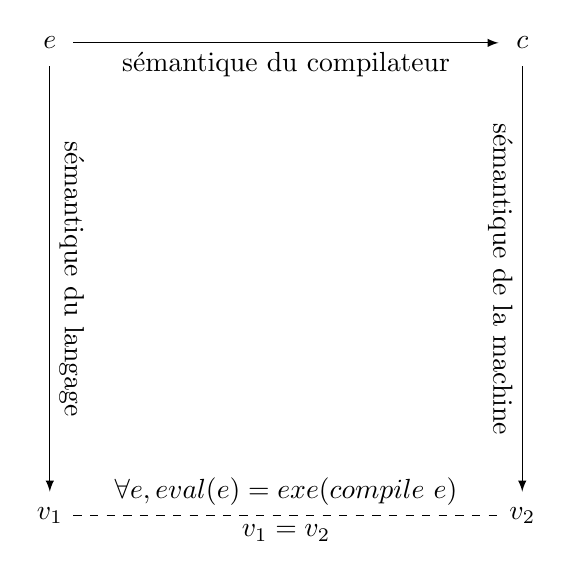
\begin{tikzpicture}
 \node at(0,6) {$e$} ;
 \node at(6,6) {$c$} ;
 \node at(6,0) {$v_2$} ;
 \node at(0,0) {$v_1$} ;
\draw[dashed] (0.3,0) -- node[below]{$v_1=v_2$} node[above]{$\forall e, eval(e)= exe(compile\ e)$}(5.7,0)  ;
\draw[-latex] (6,5.7) -- node[rotate=-90, below]{sémantique de la machine } (6,0.3) ;
\draw[-latex] (0.3,6) -- node[below]{sémantique du compilateur } (5.7,6) ;
\draw[-latex] (0,5.7) -- node[rotate=-90, above]{sémantique du langage } (0,0.3);
\end{tikzpicture}
\end{center}

\vspace{0.5cm}
%%%%%%%%%%%%%%%%%%%%%%%%%%%%%%%%%%%%%%%%%%%%%%%%%%%%%%%%%%%%%%%%%
%% This file has been automatically generated with the command
%% coqdoc --latex premier.v 
%%%%%%%%%%%%%%%%%%%%%%%%%%%%%%%%%%%%%%%%%%%%%%%%%%%%%%%%%%%%%%%%%


\begin{coqdoccode}
\coqdocnoindent
\coqdockw{Require} \coqdockw{Import} \coqdocvar{Arith}.\coqdoceol
\coqdocnoindent
\coqdockw{Require} \coqdockw{Import} \coqdocvar{ZArith}.\coqdoceol
\coqdocnoindent
\coqdockw{Require} \coqdockw{Import} \coqdocvar{Bool}.\coqdoceol
\coqdocnoindent
\coqdockw{Require} \coqdockw{Import} \coqdocvar{List}.\coqdoceol
\coqdocemptyline
\coqdocnoindent
\coqdockw{Inductive} \coqdocvar{exp} : \coqdockw{Set} :=\coqdoceol
\coqdocindent{1.00em}
\ensuremath{|} \coqdocvar{Const} : \coqdocvar{nat} \ensuremath{\rightarrow} \coqdocvar{exp}\coqdoceol
\coqdocindent{1.00em}
\ensuremath{|} \coqdocvar{Fois} : \coqdocvar{exp} \ensuremath{\rightarrow} \coqdocvar{exp} \ensuremath{\rightarrow} \coqdocvar{exp}\coqdoceol
\coqdocindent{1.00em}
\ensuremath{|} \coqdocvar{Plus} : \coqdocvar{exp} \ensuremath{\rightarrow} \coqdocvar{exp} \ensuremath{\rightarrow} \coqdocvar{exp}.\coqdoceol
\coqdocemptyline
\coqdocnoindent
\coqdockw{Fixpoint} \coqdocvar{expEval} (\coqdocvar{e}:\coqdocvar{exp}) : \coqdocvar{nat} :=\coqdoceol
\coqdocindent{1.00em}
\coqdockw{match} \coqdocvar{e} \coqdockw{with}\coqdoceol
\coqdocindent{1.00em}
\ensuremath{|} \coqdocvar{Const} \coqdocvar{n} \ensuremath{\Rightarrow} \coqdocvar{n}\coqdoceol
\coqdocindent{1.00em}
\ensuremath{|} \coqdocvar{Fois} \coqdocvar{e1} \coqdocvar{e2} \ensuremath{\Rightarrow} \coqdocvar{mult}  (\coqdocvar{expEval} \coqdocvar{e1}) (\coqdocvar{expEval} \coqdocvar{e2})\coqdoceol
\coqdocindent{1.00em}
\ensuremath{|} \coqdocvar{Plus} \coqdocvar{e1} \coqdocvar{e2} \ensuremath{\Rightarrow} \coqdocvar{plus} (\coqdocvar{expEval} \coqdocvar{e1}) (\coqdocvar{expEval} \coqdocvar{e2})\coqdoceol
\coqdocindent{1.00em}
\coqdockw{end}.\coqdoceol
\coqdocemptyline
\coqdocnoindent
\coqdockw{Inductive} \coqdocvar{instr} : \coqdockw{Set} :=\coqdoceol
\coqdocindent{0.50em}
\ensuremath{|} \coqdocvar{EMPILER} : \coqdocvar{nat} \ensuremath{\rightarrow} \coqdocvar{instr}\coqdoceol
\coqdocindent{0.50em}
\ensuremath{|} \coqdocvar{ADD} :  \coqdocvar{instr}\coqdoceol
\coqdocindent{0.50em}
\ensuremath{|} \coqdocvar{MUL} : \coqdocvar{instr}\coqdoceol
\coqdocnoindent
.\coqdoceol
\coqdocemptyline
\coqdocnoindent
\coqdockw{Definition} \coqdocvar{programme} := \coqdocvar{list} \coqdocvar{instr}.\coqdoceol
\coqdocnoindent
\coqdockw{Definition} \coqdocvar{pile} := \coqdocvar{list} \coqdocvar{nat}.\coqdoceol
\coqdocemptyline
\coqdocnoindent
\coqdockw{Definition} \coqdocvar{instrExec} (\coqdocvar{i}:\coqdocvar{instr}) (\coqdocvar{s}: \coqdocvar{pile}) : \coqdocvar{option} \coqdocvar{pile}:=\coqdoceol
\coqdocindent{1.00em}
\coqdockw{match} \coqdocvar{i} \coqdockw{with}\coqdoceol
\coqdocindent{1.00em}
\ensuremath{|} \coqdocvar{EMPILER} \coqdocvar{n} \ensuremath{\Rightarrow} \coqdocvar{Some} (\coqdocvar{n} :: \coqdocvar{s})\coqdoceol
\coqdocindent{1.00em}
\ensuremath{|} \coqdocvar{ADD} \ensuremath{\Rightarrow} \coqdoceol
\coqdocindent{2.50em}
\coqdockw{match} \coqdocvar{s} \coqdockw{with}\coqdoceol
\coqdocindent{2.50em}
\ensuremath{|} \coqdocvar{arg1} :: \coqdocvar{arg2} :: \coqdocvar{s'} \ensuremath{\Rightarrow} \coqdocvar{Some} (\coqdocvar{expEval} (\coqdocvar{Plus} (\coqdocvar{Const}(\coqdocvar{arg1})) (\coqdocvar{Const}(\coqdocvar{arg2}))) :: \coqdocvar{s'})\coqdoceol
\coqdocindent{2.50em}
\ensuremath{|} \coqdocvar{\_} \ensuremath{\Rightarrow} \coqdocvar{None}\coqdoceol
\coqdocindent{2.50em}
\coqdockw{end}\coqdoceol
\coqdocindent{1.00em}
\ensuremath{|} \coqdocvar{MUL} \ensuremath{\Rightarrow}\coqdoceol
\coqdocindent{2.50em}
\coqdockw{match} \coqdocvar{s} \coqdockw{with}\coqdoceol
\coqdocindent{2.50em}
\ensuremath{|} \coqdocvar{arg1} :: \coqdocvar{arg2} :: \coqdocvar{s'} \ensuremath{\Rightarrow} \coqdocvar{Some} (\coqdocvar{expEval} (\coqdocvar{Fois} (\coqdocvar{Const}(\coqdocvar{arg1})) (\coqdocvar{Const}(\coqdocvar{arg2}))) ::\coqdocvar{s'})\coqdoceol
\coqdocindent{2.50em}
\ensuremath{|} \coqdocvar{\_} \ensuremath{\Rightarrow} \coqdocvar{None}\coqdoceol
\coqdocindent{2.50em}
\coqdockw{end}\coqdoceol
\coqdocindent{1.00em}
\coqdockw{end}.\coqdoceol
\coqdocemptyline
\coqdocnoindent
\coqdockw{Fixpoint} \coqdocvar{progExec} (\coqdocvar{p}:\coqdocvar{programme})  (\coqdocvar{s}:\coqdocvar{pile}) : \coqdocvar{option} \coqdocvar{pile} :=\coqdoceol
\coqdocindent{1.00em}
\coqdockw{match} \coqdocvar{p} \coqdockw{with} \coqdoceol
\coqdocindent{1.00em}
\ensuremath{|} \coqdocvar{nil} \ensuremath{\Rightarrow} \coqdocvar{Some} \coqdocvar{s}\coqdoceol
\coqdocindent{1.00em}
\ensuremath{|} \coqdocvar{i} :: \coqdocvar{p'} \ensuremath{\Rightarrow} \coqdoceol
\coqdocindent{3.00em}
\coqdockw{match} \coqdocvar{instrExec} \coqdocvar{i} \coqdocvar{s} \coqdockw{with}\coqdoceol
\coqdocindent{3.00em}
\ensuremath{|} \coqdocvar{None} \ensuremath{\Rightarrow} \coqdocvar{None}\coqdoceol
\coqdocindent{3.00em}
\ensuremath{|} \coqdocvar{Some} \coqdocvar{s'} \ensuremath{\Rightarrow} \coqdocvar{progExec} \coqdocvar{p'} \coqdocvar{s'} \coqdoceol
\coqdocindent{3.00em}
\coqdockw{end}\coqdoceol
\coqdocindent{1.00em}
\coqdockw{end}.\coqdoceol
\coqdocemptyline
\coqdocnoindent
\coqdockw{Fixpoint} \coqdocvar{compile} (\coqdocvar{e}:\coqdocvar{exp}) : \coqdocvar{programme} :=\coqdoceol
\coqdocindent{1.00em}
\coqdockw{match} \coqdocvar{e} \coqdockw{with} \coqdoceol
\coqdocindent{1.00em}
\ensuremath{|} \coqdocvar{Const} \coqdocvar{n} \ensuremath{\Rightarrow} \coqdocvar{EMPILER} \coqdocvar{n} :: \coqdocvar{nil}\coqdoceol
\coqdocindent{1.00em}
\ensuremath{|} \coqdocvar{Plus} \coqdocvar{e1} \coqdocvar{e2} \ensuremath{\Rightarrow} \coqdocvar{compile} \coqdocvar{e2} ++ \coqdocvar{compile} \coqdocvar{e1} ++ \coqdocvar{ADD} :: \coqdocvar{nil}\coqdoceol
\coqdocindent{1.00em}
\ensuremath{|} \coqdocvar{Fois} \coqdocvar{e1} \coqdocvar{e2} \ensuremath{\Rightarrow} \coqdocvar{compile} \coqdocvar{e2} ++ \coqdocvar{compile} \coqdocvar{e1} ++ \coqdocvar{MUL} :: \coqdocvar{nil}\coqdoceol
\coqdocindent{1.00em}
\coqdockw{end} .\coqdoceol
\coqdocemptyline
\coqdocnoindent
\coqdockw{Eval} \coqdoctac{compute} \coqdoctac{in} (\coqdocvar{compile} (\coqdocvar{Const} 1999)) .\coqdoceol
\coqdocnoindent
\coqdockw{Eval} \coqdoctac{compute} \coqdoctac{in} (\coqdocvar{compile} (\coqdocvar{Fois} (\coqdocvar{Plus} (\coqdocvar{Const} 1999) (\coqdocvar{Const} 1)) (\coqdocvar{Const} 5))) .\coqdoceol
\coqdocnoindent
\coqdockw{Eval} \coqdoctac{compute} \coqdoctac{in} ( \coqdocvar{progExec} (\coqdocvar{compile} (\coqdocvar{Fois} (\coqdocvar{Plus} (\coqdocvar{Const} 1999) (\coqdocvar{Const} 1)) (\coqdocvar{Const} 5))) \coqdocvar{nil}) .\coqdoceol
\coqdocemptyline
\coqdocnoindent
\coqdockw{Lemma} \coqdocvar{compile\_correct\_lemme}: \coqdockw{\ensuremath{\forall}} (\coqdocvar{e}:\coqdocvar{exp}) (\coqdocvar{p}: \coqdocvar{programme}) (\coqdocvar{s}: \coqdocvar{pile}),\coqdoceol
\coqdocindent{14.00em}
\coqdocvar{progExec} (\coqdocvar{compile} \coqdocvar{e}++\coqdocvar{p}) \coqdocvar{s} = \coqdocvar{progExec} \coqdocvar{p} (\coqdocvar{expEval} \coqdocvar{e}::\coqdocvar{s})\coqdoceol
\coqdocindent{0.50em}
.\coqdoceol
\coqdocindent{0.50em}
\coqdoctac{induction} \coqdocvar{e}.\coqdoceol
\coqdocindent{0.50em}
\coqdoctac{intros}.\coqdoceol
\coqdocindent{0.50em}
\coqdoctac{unfold} \coqdocvar{compile}.\coqdoceol
\coqdocindent{0.50em}
\coqdoctac{unfold} \coqdocvar{expEval}.\coqdoceol
\coqdocindent{0.50em}
\coqdoctac{unfold} \coqdocvar{progExec} \coqdoctac{at} 1.\coqdoceol
\coqdocindent{0.50em}
\coqdoctac{simpl}.\coqdoceol
\coqdocindent{0.50em}
\coqdoctac{fold} \coqdocvar{progExec}.\coqdoceol
\coqdocindent{0.50em}
\coqdoctac{reflexivity}.\coqdoceol
\coqdocemptyline
\coqdocindent{0.50em}
\coqdoctac{intros}.\coqdoceol
\coqdocindent{0.50em}
\coqdoctac{unfold} \coqdocvar{compile}. \coqdoctac{fold} \coqdocvar{compile}.\coqdoceol
\coqdocindent{0.50em}
\coqdoctac{unfold} \coqdocvar{expEval}. \coqdoctac{fold} \coqdocvar{expEval}.\coqdoceol
\coqdocindent{0.50em}
\coqdoctac{rewrite} \coqdocvar{app\_assoc\_reverse}.\coqdoceol
\coqdocindent{0.50em}
\coqdoctac{rewrite} \coqdocvar{IHe2}. \coqdoctac{rewrite} \coqdocvar{app\_assoc\_reverse}.\coqdoceol
\coqdocindent{0.50em}
\coqdoctac{rewrite} \coqdocvar{IHe1}.\coqdoceol
\coqdocindent{0.50em}
\coqdoctac{unfold} \coqdocvar{progExec} \coqdoctac{at} 1. \coqdoctac{simpl}. \coqdoctac{fold} \coqdocvar{progExec}. \coqdoctac{reflexivity}.\coqdoceol
\coqdocemptyline
\coqdocindent{0.50em}
\coqdoctac{intros}.\coqdoceol
\coqdocindent{0.50em}
\coqdoctac{unfold} \coqdocvar{compile}. \coqdoctac{fold} \coqdocvar{compile}.\coqdoceol
\coqdocindent{0.50em}
\coqdoctac{rewrite} \coqdocvar{app\_assoc\_reverse}. \coqdoctac{rewrite} \coqdocvar{IHe2}.\coqdoceol
\coqdocindent{0.50em}
\coqdoctac{rewrite} \coqdocvar{app\_assoc\_reverse}.\coqdoceol
\coqdocindent{0.50em}
\coqdoctac{unfold} \coqdocvar{progExec} \coqdoctac{at} 1. \coqdoctac{simpl}. \coqdoctac{fold} \coqdocvar{progExec}.\coqdoceol
\coqdocindent{0.50em}
\coqdoctac{rewrite} \coqdocvar{IHe1}.\coqdoceol
\coqdocindent{0.50em}
\coqdoctac{unfold} \coqdocvar{progExec} \coqdoctac{at} 1. \coqdoctac{simpl}. \coqdoctac{fold} \coqdocvar{progExec}. \coqdoctac{reflexivity}.\coqdoceol
\coqdocemptyline
\coqdocindent{0.50em}
\coqdockw{Qed}.\coqdoceol
\coqdocemptyline
\coqdocnoindent
\coqdockw{Theorem} \coqdocvar{compile\_correct}: \coqdockw{\ensuremath{\forall}} \coqdocvar{e} : \coqdocvar{exp}, \coqdocvar{Some} ((\coqdocvar{expEval} \coqdocvar{e}) :: \coqdocvar{nil}) = (\coqdocvar{progExec} (\coqdocvar{compile} \coqdocvar{e}) \coqdocvar{nil}).\coqdoceol
\coqdocnoindent
\coqdoctac{intros}.\coqdoceol
\coqdocnoindent
\coqdoctac{rewrite} (\coqdocvar{app\_nil\_end} (\coqdocvar{compile} \coqdocvar{e})).\coqdoceol
\coqdocnoindent
\coqdoctac{rewrite} \coqdocvar{compile\_correct\_lemme}.\coqdoceol
\coqdocnoindent
\coqdoctac{reflexivity}.\coqdoceol
\coqdocnoindent
\coqdockw{Qed}.\coqdoceol
\coqdocemptyline
\coqdocnoindent
\coqdockw{Print} \coqdocvar{compile\_correct}.\coqdoceol
\end{coqdoccode}


\section{Compilation du \textsc{Lisp} vers une machine abstraite}
\subsubsection{La machine SECD}
La machine SECD inventée par Landin est une machine abstraite utilisant quatre composants:
\begin{itemize}
  \item S, la pile ou \textit{stack} permettant de stocker les résultats intermédiaires puis le résultat final
  \item E, l'environnement d'éxecution
  \item C, le code
  \item D, le dump permettant de stocker les valeurs courantes S,E,C le temps d'un calcul local d'une fonction
\end{itemize}
Nous devons implémenter deux fonctions.

La fonction de compilation \verb+compile+ qui prend en argument une expression LISP, 
un environnement de compilation et l'accumulateur du code compilé.
Nous ferons travailler la fonction \verb+compile+ sur la syntaxe abstraite pour plus de facilité.


La fonction d'éxecution  \verb+exe s e c d+  prend en arguments les 
quatre composantes de la machine abstraite.

\subsubsection{La compilation $C: exp$\ \imp\ \texttt{code}}
\noindent
  \texttt{c} \imp\ \texttt{CONST}$(c)$ \\
  \texttt{n} \imp\ \texttt{ACCESS}$(n)$ \\
  \texttt{(+ a1 a2)} \imp\ $C(a_1); C(a_2);$ \texttt{ADD} \\
  \texttt{(- a1 a2)} \imp\ $C(a_1); C(a_2);$ \texttt{SUB} \\
  \texttt{(= a1 a2)} \imp\ $C(a_1); C(a_2);$ \texttt{CMP} \\
  \texttt{((lambda (v1...vn) body) e1...en)} 
    \imp\ \texttt{NIL;} $C(v_1)$\texttt{;ARG;}$\dots C(v_n)$\texttt{;ARG;CLOSURE}$(C(body)$\texttt{;RTS}$)$\texttt{;JSR} \\
  

\subsubsection{La table de transition de la machine SECD}
\begin{footnotesize}
\[
\begin{array}{|c|c|c|c || c|c|c|c|}
  \hline
  \multicolumn{4}{|c||}{\textbf{état avant}} & \multicolumn{4}{c|}{\textbf{état après}} \\
  \hline \hline
  S & E & C & D & S & E & C & D \\
  \hline
  
  s         & e & \texttt{CONST}(cst); c & d                & cst.s         & e & c &  d \\
  n_2.n_1.s & e & \texttt{ADD}; c        & d                & (n_1 + n_2).s & e & c &  d \\
  n_2.n_1.s & e & \texttt{SUB}; c        & d                & (n_1 - n_2).s & e & c &  d \\
  n_2.n_1.s & e & \texttt{CMP}; c        & d                & (n_1 = n_2).s & e & c &  d \\
        s   & e & \mathtt{ACCESS}(n);c   & d                & e(n).s        & e & c &  d \\ 
  \hline \hline
  \multicolumn{8}{|c|}{\textrm{construction d'une liste d'arguments}} \\
  \hline
  s         & e & \mathtt{NIL}; c        & d                & [\ ]   & e & c &  d \\
  v_1.v_2.s & e & \mathtt{ARG}; c        & d                & v_1 @ v_2 . s & e & c &  d \\
  \hline \hline
  \multicolumn{8}{|c|}{\textrm{la conditionnelle}} \\
  \hline
  v.s       & e & \mathtt{BRANCH}(c_1, c_2);c & d             & s             & e & c_1;c & d \\
  v.s       & e & \mathtt{BRANCH}(c_1, c_2);c & d             & s             & e & c_2;c & d \\
  \hline \hline
  \multicolumn{8}{|c|}{\textrm{le traitement d'une clôture}} \\
  \hline
  s         & e &  \mathtt{CLOSURE}(f);c      & d             & \mathtt{CLOS}(f,e) & e & c & d \\
  \hline \hline 
  \multicolumn{8}{|c|}{\textrm{application d'une lambda avec les instructions }\texttt{JSR,RTS}} \\
  \hline 
  \mathtt{CLOS}(f,e_0).largs.s & e & \mathtt{JSR};c & d       & [\ ] & largs::e_0 & f & \mathtt{ENVEXE}(s,e,c).d \\
  v.s & e & \mathtt{RTS};c & \mathtt{ENVEXE}(s_1, e_1, c_1).d & v.s_1 & e_1 & c_1 & d \\     
  \hline
\end{array}
\]

\end{footnotesize}

\subsubsection{L'implémentation en \textsc{Ocaml}}

\begin{footnotesize}
\begin{Verbatim}
let rec compile envc exp codesuivant  =
  match exp with
  | Atom (Entier n) -> CONST n :: codesuivant
  | Var s -> ACCESS (adresse s envc) :: codesuivant
  | Call (f, args) -> compile_call envc f args codesuivant
  | Let (decl,expl) -> compile_let envc decl expl codesuivant 
  | If (cond, exp1, exp2) -> compile_if envc cond exp1 exp2 codesuivant
  | Lambda (parl, bodyl) -> compile_lambda envc parl bodyl codesuivant
  | _ -> raise (Erreur "compile")

and compile_lambda envc parl bodyl codesuivant =
  (CLOSURE ((compile (parl::envc) (hd bodyl)  [RTS])) ) :: codesuivant 

and compile_if envc cond exp1 exp2 codesuivant =
   let code_si = compile envc exp1 codesuivant
   and code_sinon = compile envc exp2 codesuivant
in compile envc cond ( BRANCH(code_si,  code_sinon) :: codesuivant ) 

and compile_call envc f args codesuivant  =
match f with 
 | Var "+" -> compile_app  envc args  (ADD :: codesuivant)
 | Var  "-"  -> compile_app  envc args  (SUB :: codesuivant)
 | Var  "="  -> compile_app  envc args  (CMP :: codesuivant)
 | _ -> compile_larg envc args (compile envc f (JSR :: codesuivant))
 
and
compile_app envc args codesuivant =
  if args = [] then codesuivant
  else  compile envc (hd args) (compile_app envc (tl args) codesuivant) 
and compile_let envc decl expl codesuivant =
  let lvar = map fst decl
  in let lexp = map snd decl
  in compile envc (Call(Lambda(lvar, expl),lexp)) codesuivant 
and compile_larg envc lexp codesuivant =
  let rec aux lexp codesuivant =
    match lexp with
    | [] -> codesuivant
    | a::b -> aux b (compile envc a (ARG::codesuivant))
  in NIL::(aux lexp codesuivant)
    
let rec exe s e c d =
  if (List.length c) = 0 then hd s
  else
    match (hd c) with
  | ADD ->  let Entier(n2) = hd (hd s) and Entier(n1) = hd (hd (tl s)) in
              exe ([Entier(n1+n2)]:: (tl (tl s))) e (tl c) d  
  | SUB ->  let Entier(n2) = hd (hd s) and Entier(n1) = hd (hd (tl s)) in
              exe ([Entier(n1-n2)]:: (tl (tl s))) e (tl c) d  
  | CMP ->  let Entier(n2) = hd (hd s) and Entier(n1) = hd (hd (tl s)) in 
                exe ([Booleen(n1=n2)]:: (tl (tl s))) e (tl c) d   
  | CONST n ->  exe ([Entier n]::s)  e (tl c) d
  | NIL ->  exe ([]::s) e (tl c) d 
  | ARG ->    let v1 = hd s
              in let v2 = hd (tl s)
                in  exe ((v1 @ v2)::(tl (tl s))) e (tl c) d
  | ACCESS sy ->  exe ([lire_env sy e]::s) e (List.tl c) d
  | BRANCH(code_si, code_sinon) ->
          let v = hd (hd s) in 
                if (v = Booleen(true)) then exe (tl s) e (code_si @ (tl c)) d 
                else exe (tl s) e ( code_sinon @ (tl c)) d 
  | CLOSURE(fonc) ->  exe ([CLOS(fonc,e)]::s) e (tl c) d
  | JSR -> let CLOS(corps, e0) = hd (hd s) in
            let larg = hd (tl s) in 
              exe [] (larg::e) corps ((ENVEXE(tl (tl s), e, (tl c)))::d) 
  | RTS -> let ENVEXE(s1, e1, c1) = hd d 
            and v = hd s in
            exe (v::s1) e1 c1 (tl d)
\end{Verbatim}
\end{footnotesize}